%%% 
%% Project Management :: Allocation of Work 
%%% 
\section{Allocation of Work}
\label{sec:allocation_of_work}

The allocation of work was primarily voluntary from members of the team. During the first term the tasks were delegated by all team members to each other clarifying on the different components that they would be working on in order to ensure there was no clash between each other. The dates for work to be completed was set by the team leader to ensure that the team was working on schedule. Tasks were delegated on a weekly basis at the group meetings. The minutes can be found in the appendix. 

Activities were split into a series of stages:

\begin{itemize}
    \item Familiarization
    \item Planning and preparation
    \item Implementation
    \item Completion
\end{itemize}

During the familiarization stage the individual members of the group got to know each other very quickly because the members have been studying on the same course over the period of 2009 to 2013 although this is the first time that all members worked together on a single project. The group initially took the time to identify areas of interest and the skills they have, which brought a sense of the strengths and weaknesses of the group.

For the planning and preparation stage the initial plans were drawn up by the group and each member stated what they thought is required to be done. Elements of the initial tasks were agreed by team members and the project supervisor. The main planning from here forward was managed by the team leader and agreed upon by the team members. Effective communication was addressed through the use of the Social Media website Facebook although more formal tools were used such as email and OneDrive(SkyDrive). During implementation the use of a version control system (GitHub) enabled the team to manage workloads effectively and track remaining issues that coincide with the project plan. The total number of issues raised was 66 although not all issues according to the project plan were raised as they were done earlier then planned. 

\begin{figure}[H]
  \centering
  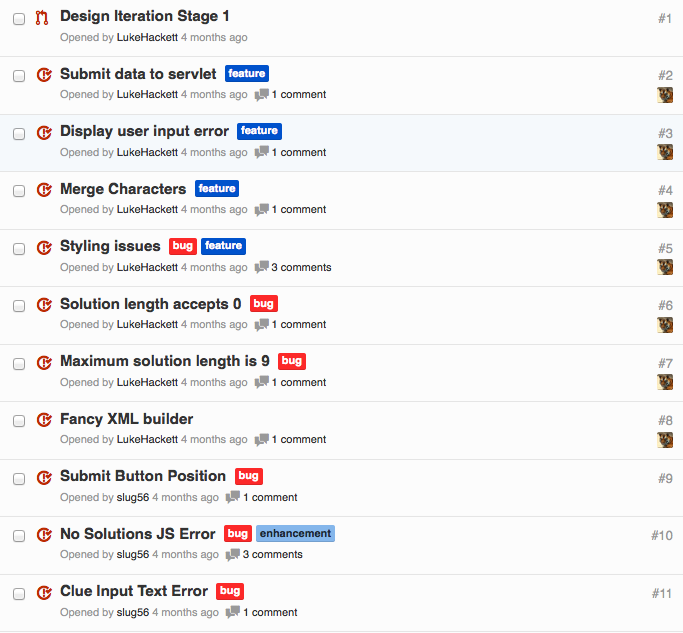
\includegraphics[width=\linewidth]{images/issues1.png}
  \caption{Issues}
  \label{fig:Issues}
\end{figure}

The tasks in the first term mainly focused upon individuals to be issued the task and produce the work by the following week and to be reviewed by the rest of the team members in the meetings. By the second term when development started the tasks were delegated to be worked in pairs. The architecture of the system was primarily developed by Stuart Leader and interfaces by Luke Hackett but in collaboration with the remainder of the team members. After the architecture of the system had been produced each team member selected a task such as a solver and attempted to write the algorithms. For the low level clues an individual was able to produce the algorithms but for the further solvers the team had to collaborate and work together.

Finally during the documentation and report writing most of the report was produced in parallel to term one and the research. Returning to the report after development proved to be beneficial as team members were once again able to select components which required to be done and produce the work. Each produced work has been throughly checked over by the other team members to ensure that anything that has been produced and written is up to its standards.